%% Overleaf			
%% Software Manual and Technical Document Template	
%% 									
%% This provides an example of a software manual created in Overleaf.

\documentclass{../ol-softwaremanual}

% Packages used in this example
\usepackage{graphicx}  % for including images
\usepackage{microtype} % for typographical enhancements
\usepackage{minted}    % for code listings
\usepackage{amsmath}   % for equations and mathematics
\setminted{style=friendly,fontsize=\small}
\renewcommand{\listoflistingscaption}{List of Code Listings}
\usepackage{hyperref}  % for hyperlinks
\usepackage[a4paper,top=4.2cm,bottom=4.2cm,left=3.5cm,right=3.5cm]{geometry} % for setting page size and margins

\usepackage[english, greek]{babel}

\usepackage{subfig}




% Custom macros used in this example document
\newcommand{\doclink}[2]{\href{#1}{#2}\footnote{\url{#1}}}
\newcommand{\cs}[1]{\texttt{\textbackslash #1}}

\begin{document}
	
	
	\begin{titlepage}
		
		
		% Frontmatter data; appears on title page
		\title{\en Class Diagram \\}
		\version{0.1}
		\softwarelogo{
\includegraphics[scale=0.4]{../CarBazaar_logo.png}}
	\end{titlepage}
	
	
	\maketitle
	
	\newpage
	
	\center{\textbf{Μέλη Ομάδας}}
	
	\vspace{20pt}
	
	
	
	\begin{table}[htbp!]
		
		\begin{tabular}{llll}
			Μεμελετζόγλου Χαρίλαος & 1069364 & \en st1069364@ceid.upatras.gr & 4o Έτος   \\ 
			\\ Λέκκας Γεώργιος      &      1067430    &   \en st1067430@ceid.upatras.gr & 4o Έτος  \\
			\\ Γιαννουλάκης Ανδρέας        &   1067387       & \en st1067387@ceid.upatras.gr & 4o Έτος           \\
			\\ Κανελλόπουλος Ιωακείμ        &  1070914        &    \en st1070914@ceid.upatras.gr & 4o Έτος        \\ 
		\end{tabular}
	\end{table}
	
	\center{\textbf{Υπεύθυνοι Παρόντος Τεχνικού Κειμένου}}
	
	\vspace{20pt}
	
	\begin{table}[htbp!]
		\begin{tabular}{ll}
			Μεμελετζόγλου Χαρίλαος & \en Editor \\
			\\ Λέκκας Γεώργιος      &   \en  Editor \\
			\\ Γιαννουλάκης Ανδρέας & \en Peer Reviewer \\
			\\ Κανελλόπουλος Ιωακείμ & \en Peer Reviewer \\ 
		\end{tabular}
	\end{table}
		
	\newpage 
	
	
	\center{\textbf{Εργαλεία που χρησιμοποιήθηκαν}}
	
	\vspace{20pt}
	\flushleft
	Χρησιμοποιήθηκε το \en \doclink{https://www.overleaf.com/}{Overleaf} \gr και το \en \doclink{https://www.texstudio.org/}{TexStudio} \gr για την συγγραφή του \LaTeX\ κώδικα. \break
	
	Για την δημιουργία του \en Class Diagram \gr χρησιμοποιήθηκε το \en \doclink{https://www.visual-paradigm.com/}{Visual Paradigm} \gr .
	
	\newpage
	
	\center{\textbf{\en Class Diagram \gr}}
	
	\begin{figure}[htbp!]		
		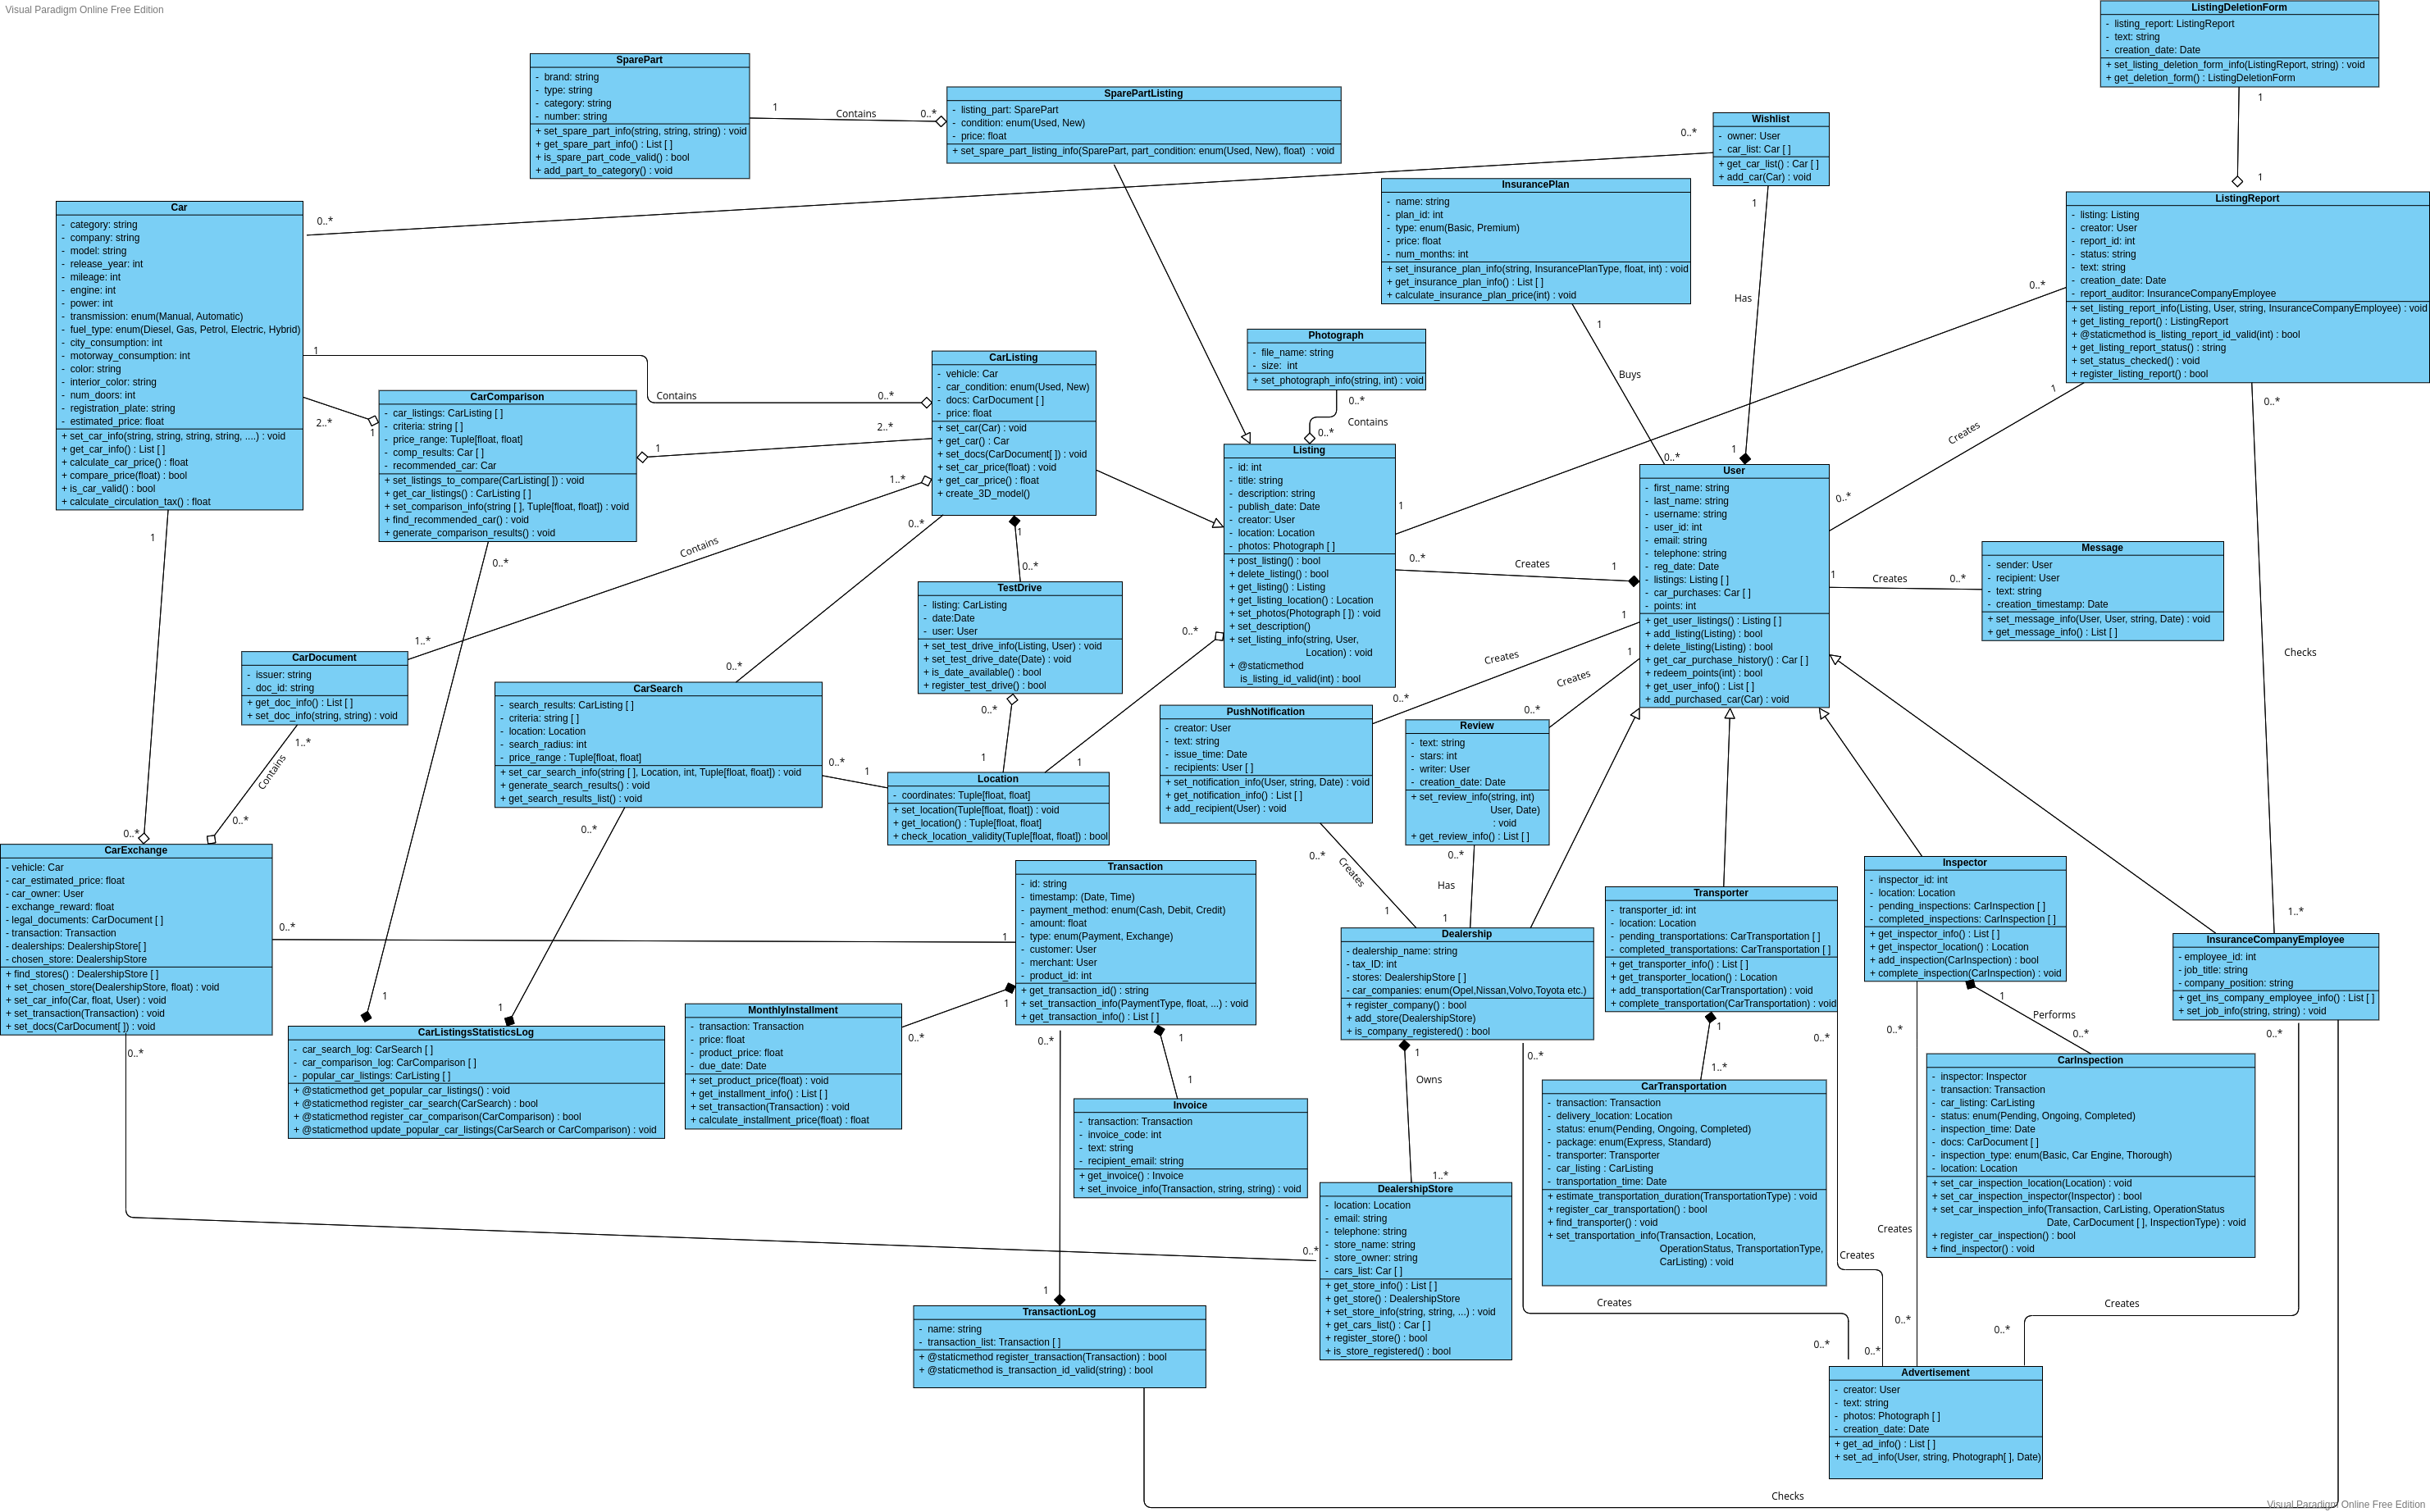
\includegraphics[width=\textwidth+3.4cm, height=15cm]{img/class_diagram_v0.1.png}
		\caption{\en UML Class Diagram \gr του \en Project \gr}
	\end{figure}
	
	
	
	\newpage
	
	\center{\textbf{Περιγραφή Κλάσεων}}
	
	\begin{itemize}
		\item \en \textbf{Car} \gr : Οντότητα που αντιστοιχεί σε ένα αυτοκίνητο και περιέχει όλα τα χαρακτηριστικά του (έτος κυκλοφορίας, μοντέλο κλπ)		
		\item \en \textbf{SparePart} \gr : Οντότητα που αντιστοιχεί σε ένα ανταλλακτικό και περιέχει όλα τα χαρακτηριστικά του
		\item \en \textbf{User} \gr : Γενική Οντότητα που αντιστοιχεί στον εγγεγραμμένο χρήστη της πλατφόρμας. Περιέχει χαρακτηριστικά του χρήστη, όπως το ονοματεπώνυμο, το \en username \gr, τον κωδικό του, το \en email \gr του, το τηλέφωνό του και την ημερομηνία εγγραφής του
		\item \en \textbf{Inspector} \gr : Ειδικότερη περίπτωση εγγεγραμμένου χρήστη, που αντιστοιχεί στους Ελεγκτές που διεξάγουν τους ελέγχους των οχημάτων. Περιέχει τον κωδικό του Ελεγκτή, την τοποθεσία του, καθώς και μια την λίστα με τους εκκρεμείς αλλά και ολοκληρωμένους ελέγχους οχημάτων του συγκεκριμένου Ελεγκτή
		\item \en \textbf{Transporter} \gr : Ειδικότερη περίπτωση εγγεγραμμένου χρήστη, που αφορά τους Μεταφορείς, ευθύνη των οποίων είναι η μεταφορά οχημάτων. Περιέχει τον κωδικό του Μεταφορέα, την μόνιμη τοποθεσία του Μεταφορέα, καθώς και μια την λίστα με τις εκκρεμείς αλλά και ολοκληρωμένες μεταφορές οχημάτων του συγκεκριμένου Μεταφορέα
		\item \en \textbf{Dealership} \gr : Ειδικότερη περίπτωση εγγεγραμμένου χρήστη, που αντιστοιχεί σε μια Αντιπροσωπεία Οχημάτων. Περιέχει πληροφορίες όπως το όνομα της εταιρείας, τον Αριθμό Φορολογικού Μητρώου της, μια λίστα με τα Καταστήματά της καθώς και μια λίστα με τις εταιρείες των οχημάτων που διαθέτει προς πώληση
		\item \en \textbf{InsuranceCompanyEmployee} \gr : Ειδικότερη περίπτωση εγγεγραμμένου χρήστη, που αντιστοιχεί σε υπάλληλο της Ασφαλιστικής Εταιρείας που διαχειρίζεται την πλατφόρμα. Περιέχει στοιχεία όπως, τον κωδικό του υπαλλήλου, το τμήμα της Ασφαλιστικής Εταιρείας στο οποίο εργάζεται, καθώς και τον τίτλο της θέσης του
		\item \en \textbf{Listing} \gr : Οντότητα που αντιστοιχεί σε μια αναρτημένη, στο σύστημα, αγγελία. Μπορεί να είναι είτε αγγελία πώλησης οχήματος (από Ιδιώτη ή από Αντιπροσωπεία), είτε αγγελία πώλησης ανταλλακτικού, είτε αγγελία που έχει αναρτήσει κάποιος Ελεγκτής προκειμένου να πληροφορήσει του χρήστες για τις υπηρεσίες που παρέχει. Περιέχει, μεταξύ άλλων, πληροφορίες όπως τον τίτλο της αγγελίας, τον κωδικό της και την περιγραφή της
		\item \en \textbf{CarListing} \gr : Ειδικότερη περίπτωση αναρτημένης αγγελίας, που αφορά αγγελία πώλησης οχήματος. Περιέχει το όχημα, την κατάστασή του, τα έγγραφά του και την τιμή του
		\item \en \textbf{SparePartListing} \gr : Ειδικότερη περίπτωση αναρτημένης αγγελίας, που αντιστοιχεί σε αγγελία πώλησης ανταλλακτικού. Περιέχει το ανταλλακτικό, την κατάστασή του, καθώς και την τιμή πώλησής του
		\item \en \textbf{ListingReport} \gr : Οντότητα που αντιστοιχεί σε Αναφορά αγγελίας. Περιέχει πληροφορίες όπως την υπό αναφορά αγγελία, τον χρήστη που δημιούργησε την αναφορά, τον κωδικό της αναφοράς, το κείμενο με την αιτία υποβολής της αναφοράς, την ημερομηνία δημιουργίας της και τον υπάλληλο της Ασφαλιστικής Εταιρείας που εξέτασε την αναφορά
		\item \en \textbf{ListingDeletionForm} \gr : Οντότητα που αντιστοιχεί στην φόρμα διαγραφής αγγελίας, την οποία συμπληρώνει ο υπάλληλος της ασφαλιστικής εταιρείας, που εξετάζει την αναφορά που έχει δεχθεί μια αγγελία. Περιέχει πληροφορίες όπως το κείμενο με την αιτία διαγραφής της αγγελίας, την ημερομηνία δημιουργίας της φόρμας καθώς και τις πληροφορίες της αναφοράς της αγγελίας			
		\item \en \textbf{Transaction} \gr : Οντότητα που αντιστοιχεί σε μια συναλλαγή που διεξήχθη μέσω της πλατφόρμας και περιέχει όλα τα χαρακτηριστικά της, όπως κωδικός συναλλαγής, ποσό, ημερομηνία κλπ.
		\item \en \textbf{TransactionLog} \gr : Οντότητα που αντιστοιχεί στο μοναδικό και καθολικό Αρχείο Καταγραφής συναλλαγών (\en Log\gr), στο οποίο έχει πρόσβαση μόνο η Ασφαλιστική Εταιρεία. Έχει τίτλο και μια λίστα από τις συναλλαγές που έχουν διεξαχθεί
		\item \en \textbf{Message} \gr : Οντότητα που αντιστοιχεί σε μήνυμα που αποστέλλουν μεταξύ τους οι χρήστες της εφαρμογής και περιέχει χαρακτηριστικά όπως το \en username \gr του αποστολέα και του παραλήπτη, το κείμενο του μηνύματος και την ημερομηνία και ώρα δημιουργίας του μηνύματος
		\item \en \textbf{Location} \gr : Οντότητα που περιγράφει μια φυσική τοποθεσία με βάση το γεωγραφικό της στίγμα
		\item \en \textbf{Advertisement} \gr : Οντότητα που αντιστοιχεί σε μια διαφήμιση που έχει δημιουργηθεί είτε από μια Αντιπροσωπεία, είτε από έναν Μεταφορέα, είτε από έναν Ελεγκτή, είτε από την Ασφαλιστική Εταιρεία. Περιέχει το \en username \gr του δημιουργού της, το κείμενό της, μια λίστα από φωτογραφίες καθώς και την ημερομηνία δημιουργίας της
		\item \en \textbf{PushNotification} \gr : Οντότητα που αφορά τα \en Push Notifications \gr που μπορεί να δημιουργήσει μια Αντιπροσωπεία, είτε ειδοποιήσεις που εμφανίζονται στον χρήστη, πχ ως υπενθύμιση για ένα ραντεβού για \en Test Drive \gr. Περιέχει το \en username \gr του δημιουργού της ειδοποίησης, το κείμενό της, την ημερομηνία δημιουργίας, καθώς και μια λίστα με τα \en usernames \gr των παραληπτών
		\item \en \textbf{CarDocument} \gr : Οντότητα που αντιστοιχεί σε έγγραφα ενός οχήματος (είτε νομικά είτε πιστοποίησης κατάστασης). Περιέχει το όνομα του φορέα έκδοσης και έναν μοναδικό κωδικό
		\item \en \textbf{CarExchange} \gr : Οντότητα που αφορά μια Ανταλλαγή Οχημάτων που διεξάγεται μεταξύ ενός Ιδιώτη χρήστη και μιας Αντιπροσωπείας. Περιέχει, μεταξύ άλλων, τα στοιχεία του οχήματος, τα στοιχεία του χρήστη, την ανταμοιβή του και το κατάστημα της Αντιπροσωπείας 
		\item \en \textbf{CarComparison} \gr : Οντότητα που αντιστοιχεί σε μια σύγκριση μεταξύ οχημάτων, και περιέχει στοιχεία όπως μια λίστα με τις αγγελίες των οχημάτων που συμμετέχουν στην σύγκριση, τα κριτήρια με βάση τα οποία γίνεται η σύγκριση, το εύρος τιμών, μια λίστα με τα αποτελέσματα της σύγκρισης καθώς και το προτεινόμενο από το σύστημα, όχημα
		\item \en \textbf{CarSearch} \gr : Οντότητα που αντιστοιχεί σε αναζήτησης οχήματος και περιέχει στοιχεία όπως την τοποθεσία του χρήστη, την ακτίνα αναζήτησης, μια λίστα με τις αγγελίες που συνιστούν τα αποτελέσματα της αναζήτησης, τα κριτήρια της αναζήτησης και το εύρος τιμών		
		\item \en \textbf{CarListingsStatisticsLog} \gr : Οντότητα που αντιστοιχεί στο μοναδικό και καθολικό Αρχείο Καταγραφής Αναζητήσεων και Συγκρίσεων Οχημάτων. Έχει μια λίστα από τις αναζητήσεις και συγκρίσεις οχημάτων που έχουν διεξαχθεί από τους χρήστες της πλατφόρμας, καθώς και μια λίστα με τις δημοφιλείς αγγελίες οχημάτων. Η κλάση αυτή χρησιμοποιείται προκειμένου, να μπορεί να διεξαχθεί στατιστική ανάλυση στις αναζητήσεις των χρηστών, και να εξαχθούν οι δημοφιλείς αγγελίες που εμφανίζονται συχνά στις αναζητήσεις και τις συγκρίσεις		
		\item \en \textbf{CarInspection} \gr : Οντότητα που αφορά προγραμματισμένο έλεγχο οχήματος και περιέχει, μεταξύ άλλων, στοιχεία όπως, τον Ελεγκτή που θα πραγματοποιήσει τον έλεγχο, την αγγελία του υπό εξέταση οχήματος, τον τύπο του ελέγχου κ.α.
		\item \en \textbf{CarTransporation} \gr : Οντότητα που αντιστοιχεί σε μια προγραμματισμένη μεταφορά οχήματος, και περιέχει, μεταξύ άλλων, στοιχεία όπως τον Μεταφορέα, το όχημα, τον τύπο της μεταφοράς (Κανονική ή \en Express \gr), την τοποθεσία παράδοσης του οχήματος
		\item \en \textbf{TestDrive} \gr : Οντότητα που αντιστοιχεί σε ένα προγραμματισμένο ραντεβού για \en Test Drive \gr ενός οχήματος. Περιέχει πληροφορίες όπως την αγγελία του οχήματος, την ημερομηνία του ραντεβού καθώς και τα στοιχεία του χρήστη που προγραμμάτισε το ραντεβού
		\item \en \textbf{InsurancePlan} \gr : Οντότητα που αφορά ένα Ασφαλιστικό Πακέτο και περιέχει χαρακτηριστικά όπως τον κωδικό του πακέτου, το όνομα του πακέτου, τον τύπο του, τα μηνιαία ασφάλιστρα και την διάρκεια του πακέτου σε μήνες
		\item \en \textbf{MonthlyInstallment} \gr : Οντότητα που αφορά την Μηνιαία Δόση εξόφλησης της αγοράς ενός οχήματος και περιέχει στοιχεία όπως τα στοιχεία της συναλλαγής αγοράς του οχήματος, το ποσό της δόσης και την καταληκτική ημερομηνία καταβολής της
		\item \en \textbf{Invoice} \gr : Οντότητα που αφορά την Απόδειξη Συναλλαγής. Περιέχει τις πληροφορίες της συναλλαγής, τον κωδικό της απόδειξης, το κείμενό της και το \en email \gr του παραλήπτη της	
		\item \en \textbf{Review} \gr : Οντότητα που αντιστοιχεί σε κριτική που μπορεί να έχει δεχθεί ένα Ιδιώτης ή μια Αντιπροσωπεία. Περιέχει χαρακτηριστικά όπως το κείμενο της κριτικής, τον αριθμό των αστεριών, το \en username \gr του δημιουργού, την ημερομηνία της δημιουργίας
		\item \en \textbf{Photograph} \gr : Οντότητα που αντιστοιχεί σε μια Φωτογραφία που μπορεί να είναι μέρος μιας αγγελίας πώλησης οχήματος ή ανταλλακτικού. Περιέχει το όνομα του αρχείου και το μέγεθός του σε \en Bytes \gr
		\item \en \textbf{Wishlist} \gr : Οντότητα που αντιστοιχεί στην \en Wishlist \gr ενός χρήστη. Περιέχει τα στοιχεία του κατόχου της και μια λίστα από οχήματα
		\item \en \textbf{DealershipStore} \gr : Οντότητα που αντιστοιχεί σε Φυσικό Κατάστημα που υπάγεται σε μια Αντιπροσωπεία Οχημάτων. Περιλαμβάνει, μεταξύ άλλων, στοιχεία όπως την τοποθεσία του, το όνομα του καταστήματος και μια λίστα με τα οχήματα που διαθέτει προς πώληση
	\end{itemize}
	
	
	
	
	
\end{document}
